\documentclass{article}

\usepackage{tikz}
\usetikzlibrary{arrows.meta}

% ==================================================
% COLORS
% ==================================================

\definecolor{navy}{RGB}{20,55,100}
\definecolor{blue}{RGB}{40,90,150}
\definecolor{bluepale}{RGB}{235,242,250}
\definecolor{gold}{RGB}{190,140,40}
\definecolor{goldpale}{RGB}{255,248,220}
\definecolor{green}{RGB}{45,140,85}
\definecolor{greenpale}{RGB}{230,248,238}

\begin{document}
	
	\begin{figure}[ht]
		\centering
		
		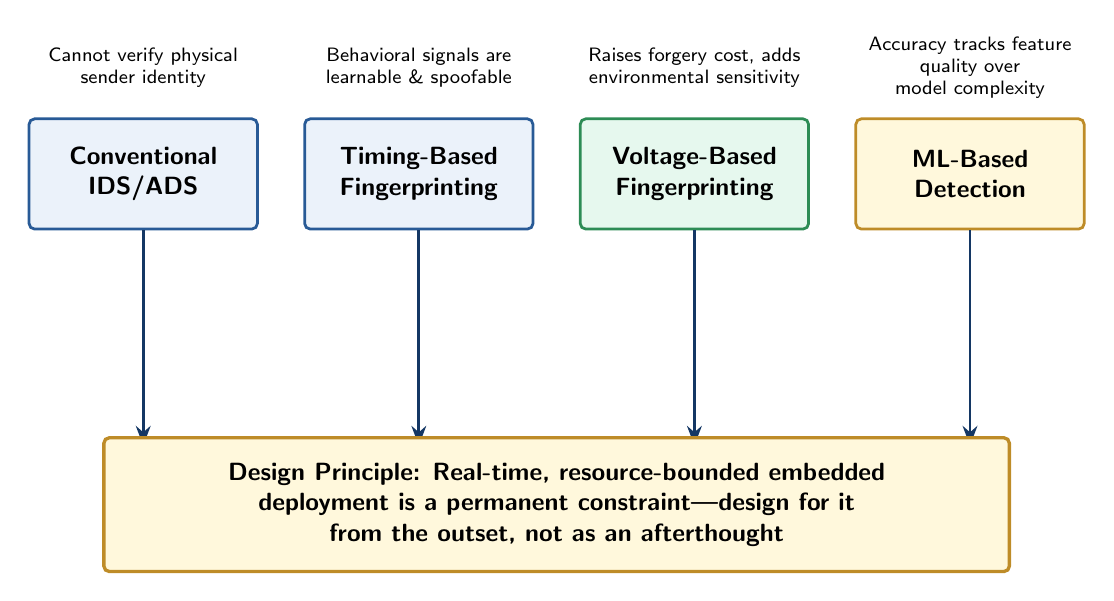
\begin{tikzpicture}[x=1cm,y=1cm]
			
			% ==================================================
			% DESCRIPTIONS ABOVE THE BOXES
			% ==================================================
			
			\node[
			font=\sffamily\scriptsize,
			text width=2.7cm,
			align=center
			] at (0,4.75)
			{Cannot verify physical\\sender identity};
			
			\node[
			font=\sffamily\scriptsize,
			text width=2.7cm,
			align=center
			] at (3.5,4.75)
			{Behavioral signals are\\learnable \& spoofable};
			
			\node[
			font=\sffamily\scriptsize,
			text width=2.7cm,
			align=center
			] at (7.0,4.75)
			{Raises forgery cost, adds\\environmental sensitivity};
			
			\node[
			font=\sffamily\scriptsize,
			text width=2.7cm,
			align=center
			] at (10.5,4.75)
			{Accuracy tracks feature\\quality over model complexity};
			
			
			% ==================================================
			% TOP BOXES
			% ==================================================
			
			\node[
			rectangle,
			rounded corners=2pt,
			draw=blue,
			fill=bluepale,
			line width=1pt,
			minimum width=2.9cm,
			minimum height=1.4cm,
			align=center,
			font=\sffamily\bfseries\small
			] (n1) at (0,3.4)
			{Conventional\\IDS/ADS};
			
			\node[
			rectangle,
			rounded corners=2pt,
			draw=blue,
			fill=bluepale,
			line width=1pt,
			minimum width=2.9cm,
			minimum height=1.4cm,
			align=center,
			font=\sffamily\bfseries\small
			] (n2) at (3.5,3.4)
			{Timing-Based\\Fingerprinting};
			
			\node[
			rectangle,
			rounded corners=2pt,
			draw=green,
			fill=greenpale,
			line width=1pt,
			minimum width=2.9cm,
			minimum height=1.4cm,
			align=center,
			font=\sffamily\bfseries\small
			] (n3) at (7.0,3.4)
			{Voltage-Based\\Fingerprinting};
			
			\node[
			rectangle,
			rounded corners=2pt,
			draw=gold,
			fill=goldpale,
			line width=1pt,
			minimum width=2.9cm,
			minimum height=1.4cm,
			align=center,
			font=\sffamily\bfseries\small
			] (n4) at (10.5,3.4)
			{ML-Based\\Detection};
			
			
			% ==================================================
			% STRAIGHT ARROWS
			% ==================================================
			
			\draw[
			-{Stealth[length=2.5mm]},
			draw=navy,
			line width=1pt
			] (n1.south) -- (0,-0.05);
			
			\draw[
			-{Stealth[length=2.5mm]},
			draw=navy,
			line width=1pt
			] (n2.south) -- (3.5,-0.05);
			
			\draw[
			-{Stealth[length=2.5mm]},
			draw=navy,
			line width=1pt
			] (n3.south) -- (7.0,-0.05);
			
			\draw[
			-{Stealth[length=2.5mm]},
			draw=navy,
			line width=1pt
			] (n4.south) -- (10.5,-0.05);
			
			
			% ==================================================
			% WIDER DESIGN PRINCIPLE BOX
			% ==================================================
			
			\node[
			rectangle,
			rounded corners=2pt,
			draw=gold,
			fill=goldpale,
			line width=1.2pt,
			minimum width=11.5cm,
			minimum height=1.7cm,
			align=center,
			font=\sffamily\bfseries\small
			] at (5.25,-0.8)
			{Design Principle: Real-time, resource-bounded embedded\\
				deployment is a permanent constraint---design for it\\
				from the outset, not as an afterthought};
			
		\end{tikzpicture}
		
		\caption{Synthesis of Lessons Learned Across the Automotive Cybersecurity and ECU Fingerprinting Literature.}
		
		\label{fig:lessons}
		
	\end{figure}
	
\end{document}